\section{Задача поддержки очереди задач IBM LSF в клиенте запуска расчетов на кластере scheduler}

% \subsection{Постановка задачи}

Постановка задачи:

\begin{enumerate}
    \item Установить и настроить IBM LSF;
    \item Поддержать API для LSF в серверной части Scheduler;
    \item Поддержать команды, направляемы напрямую из Scheduler на кластер;
    \item Протестировать.
\end{enumerate}

На блок-схеме \ref{fig:block-scheme} изображены отношения между элементами. Каждый элемент не знает о элементах за элементом, с которым он связан. Каждый элемент служит абстракцией.

\begin{figure}[h]
    \centering
    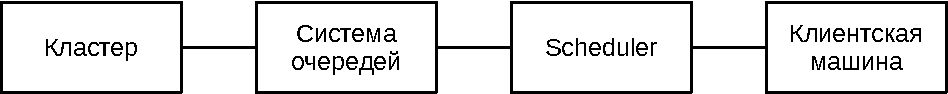
\includegraphics{scheme.pdf}
    \caption{Блок-схема}
    \label{fig:block-scheme}
\end{figure}


% \subsection{Решение} 


\subsection{Установка и настройка LSF}

% \subsection{Планировка установки}

% Plan your installation to determine the required parameters for the install.config file.
Запланируйте установку, чтобы задать необходимые параметры для файла \lstinline{install.config} \cite{install_plan}.

% Choose a primary LSF administrator (owns the LSF and EGO configuration files and log files). For example,
Укажите главный администратор LSF (владеет файлами настроек и файлами лога LSF и EGO). Например,

\begin{lstlisting}
LSF_ADMINS="lsfadmin"
\end{lstlisting}

% Choose a shared LSF installation directory. For example,
Укажите общую директорию установки LSF. Например,

\begin{lstlisting}
LSF_TOP="/usr/share/lsf"
\end{lstlisting}

% Choose LSF hosts (management host, management candidates, server hosts, and client-only hosts). For example,
Укажите хосты LSF (хост управления, хосты кандидаты в хосты управления, хосты серверы и хосты клиенты). Например,

\begin{lstlisting}
LSF_ADD_SERVERS="hostm hostb hostc hostd"
LSF_MASTER_LIST="hostm hostd"
LSF_ADD_CLIENTS="hoste hostf"
\end{lstlisting}

% Important: Do not use the name of any host, user, or user group as the name of your cluster.
Важно: не используйте имя какого-либо хоста, пользователя или группы пользователей в качестве имени вашего кластера.

% Choose LSF server hosts that are candidates to become the management host for the cluster, if you are installing a new host to be dynamically added to the cluster. For example,
Укажите хосты сервера LSF, которые являются кандидатами на роль хоста управления для кластера, если вы устанавливаете новый хост, который будет динамически добавлен в кластер. Например,

\begin{lstlisting}
LSF_MASTER_LIST="hosta hostb"
\end{lstlisting}

% Choose a cluster name that has 39 characters or less with no white spaces. For example,
Укажите имя кластера, содержащее не более 39 символов без пробелов. Например,

\begin{lstlisting}
LSF_CLUSTER_NAME="cluster1"
\end{lstlisting}

% If you are installing LSF Standard Edition, choose a configuration template to determine the initial configuration of your new cluster. For example,
Если вы устанавливаете LSF Standard Edition, выберите шаблон настройки для начальной настройки вашего нового кластера. Например,

\begin{lstlisting}
CONFIGURATION_TEMPLATE="HIGH_THROUGHPUT"
\end{lstlisting}

% Select one of the following templates, depending on the type of jobs that your cluster will run:
Выберите один из следующих шаблонов в зависимости от типа задач, которые будет выполнять ваш кластер:

\begin{itemize}
    % \item \lstinline{DEFAULT} --- Select this template for clusters with mixed workload. This configuration can serve different types of workload with good performance, but is not tuned for a particular type of cluster.
    % \item \lstinline{PARALLEL} --- Select this template for clusters that are running large parallel jobs. This configuration is designed for long running parallel jobs and not for clusters that mainly run short jobs due to the longer reporting time for each job.
    % \item \lstinline{HIGH_THROUGHPUT} --- This template is used for clusters that mainly run short jobs, where over 80\% of jobs finish within one minute. This high turnover rate requires LSF to be more responsive and fast acting, but will use more resources as the daemons become busier.
    \item \lstinline {DEFAULT} --- укажите этот шаблон для кластеров со смешанной рабочей нагрузкой. Эта конфигурация может обслуживать различные типы рабочих нагрузок с хорошей производительностью, но не настроена для конкретного типа кластера;
    \item \lstinline {PARALLEL} --- укажите этот шаблон для кластеров, в которых выполняются большие параллельные задачи. Эта конфигурация предназначена для длительных параллельных задач, а не для кластеров, которые в основном выполняют короткие задания из-за более длительного времени отчетности для каждой задачи;
    \item \lstinline {HIGH_THROUGHPUT} --- этот шаблон используется для кластеров, которые в основном выполняют короткие задания, где более 80\% заданий завершаются в течение одной минуты. Такая высокая текучесть задач требует, чтобы LSF был более отзывчивым и быстродействующим, но по мере того, как демоны становятся более загруженными, будет использовать больше ресурсов.
\end{itemize}

% Настройка значений полей в конфиг-файле \lstinline{install.config} \cite{install_plan}:
% \begin{lstlisting}
% LSF_ADMINS="lsfadmin"
% LSF_TOP="/usr/share/lsf"
% LSF_ADD_SERVERS="hostm hostb hostc hostd"
% LSF_MASTER_LIST="hostm hostd"
% LSF_ADD_CLIENTS="hoste hostf"
% LSF_CLUSTER_NAME="cluster1"
% CONFIGURATION_TEMPLATE="HIGH_THROUGHPUT"    
% \end{lstlisting}

Значение полей:

\lstinline{LSF_ADMINS}: имена пользователей администраторов LSF;

\lstinline{LSF_TOP}: полный путь директории установки LSF;

\lstinline{LSF_ADD_SERVERS}: хосты сервера, которые могут ставить задания в очередь и выполнять задания;

\lstinline{LSF_MASTER_LIST}: главный хост, который действует как всеобщий координатор для кластера. В каждом кластере есть один главный узел, который выполняет планирование и отправку всех заданий из очередей в хосты исполнения;

\lstinline{LSF_ADD_CLIENTS}: хосты клиенты, которые могут только ставить задания в очередь;

\lstinline{LSF_CLUSTER_NAME}: имя кластера LSF;

\lstinline{CONFIGURATION_TEMPLATE}: шаблон конфигурации для определения начальной конфигурации нового кластера \cite{lsf_overview, hosts_about}.

Создание пользователя для администратора LSF и запуск установки LSF:

\begin{lstlisting}
$ sudo -i
# adduser lsfadmin
# ./lsfinstall -f install.config
\end{lstlisting}

Запуск LSF:

\begin{lstlisting}
# source /usr/share/lsf/conf/profile.lsf
# lsfstartup
\end{lstlisting}

% Настройка автозапуска LSF:
Введите следующие команды, чтобы использовать кластер LSF, установленный в каталоге \lstinline{/usr/share/lsf}, и настроить демоны LSF для автоматического запуска во время запуска машины \cite{configuring-cluster}:

\begin{lstlisting}
# cd /usr/share/lsf/10.1/install
# ./hostsetup --top="/usr/share/lsf" --boot="y"
\end{lstlisting}


\lstset{emph={job_file}}
\subsection{Поддержка API для LSF в серверной части Scheduler}

Shell-скрипты формируют файл c информацией для запуска задачи, который запускается командой \lstinline{bsub} --- она считывает файл задачи, параметры в виде строк начинающихся с \lstinline{#BSUB} и запрашивает в системе очередей необходимые ресурсы, после чего задача ставится в очередь и, когда запрошенные ресурсы освобождаются, исполняется остальная часть. \lstinline{job_file} --- это shell-скрипт с прописанными директивами \lstinline{#BSUB} в начале файла.

За основу взяты шаблоны задач и скрипты bash системы очередей Torque для поддержки LSF. Шаблоны задач и скрипты Torque переписаны для LSF. Созданы shell скрипты, которые формируют файл c информацией для запуска задачи

\lstinline{run_rnkim_decomp_mpi_lsf.sh},

\lstinline{run_rnkim_mpi_lsf.sh},

\lstinline{run_rnkim_omp_lsf.sh}

и шаблоны задач

\lstinline{template_rnkim_decomp_lsf},

\lstinline{template_rnkim_decomp_mpi_lsf},

\lstinline{template_rnkim_mpi_lsf},

\lstinline{template_rnkim_omp_lsf}

для LSF.

Переписывание скриптов bash с Torque на LSF:

Отправка задачи \lstinline{job_file} в очередь 

\begin{lstlisting}
qsub job_file
-->
bsub < job_file
\end{lstlisting}
\lstset{emph={}}

В параметр \lstinline{-m} --- конкретные хосты, группы хостов, вычислительные единицы --- передаются теги или типы узлов.

\begin{lstlisting}
$NODETYPE
-->
_tmplNODETYPE_="#BSUB -m \"$NODETYPE\""
\end{lstlisting}

Переписывание шаблонов задач с Torque на LSF:

В параметр \lstinline{-n} --- задает кол-во тасков в задаче --- передается кол-во ядер в узле \lstinline{_tmplCORES_}.

В параметр \lstinline{-R} --- задает строку ресурсов --- передается кол-во узлов \lstinline{1} \cite{ref_bsub}.
\begin{lstlisting}
#PBS -l nodes=1_tmplNODETYPE_:ppn=_tmplCORES_
-->
#BSUB -n _tmplCORES_ -R "span[hosts=1]"
_tmplNODETYPE_
\end{lstlisting}

В параметр \lstinline{-n} --- задает кол-во тасков в задаче --- передается кол-во всех ядер в узлах \lstinline{_tmplTOTALCORES_}.

В параметр \lstinline{-R} --- задает строку ресурсов --- передается кол-во ядер на узел \lstinline{_tmplCORES_}.
\begin{lstlisting}
#PBS -l nodes=_tmplNNODES__tmplNODETYPE_:ppn=_tmplCORES_
-->
#BSUB -n _tmplTOTALCORES_ -R "span[ptile=_tmplCORES_]"
_tmplNODETYPE_

TOTALCORES = NNODES * CORES
\end{lstlisting}

В параметр \lstinline{-notify} --- запрашивает уведомление пользователя, когда задание достигает любого из указанных состояний --- передаются состояния программы.

В параметр \lstinline{-R} --- отправляет письмо по указанному адресу электронной почты --- передается адрес электронной почты.
\begin{lstlisting}
#PBS -m ea
#PBS -M <usermail>
-->
#BSUB -notify "exit done"
#BSUB -u <usermail>
\end{lstlisting}

В параметр \lstinline{-R} --- присваивает указанное имя заданию --- передается имя модели.

В параметр \lstinline{-W} --- устанавливает ограничение времени выполнения задания --- передается период 150 часов.

В параметр \lstinline{-cwd} --- задает текущую рабочую директорию для выполнения задания --- передается путь директории.
\begin{lstlisting}
#PBS -N _tmplMODEL_
#PBS -l walltime=150:00:00
#PBS -d _tmplDIR_
-->
#BSUB -J _tmplMODEL_
#BSUB -W 150:00
#BSUB -cwd _tmplDIR_
\end{lstlisting}


\subsection{Поддержка команд, направляемы напрямую из Scheduler на кластер}

Команды в Scheduler, относящиеся к конкретной системе очередей, хранятся в значениях ключей в словаре (тип данных на Python). Значениям соответствуют либо ссылки на исполняемые на сервере скрипты, либо команды для системы очередей, либо ссылки на методы обработки. Для LSF добавлены следующие значения ключей:
\begin{lstlisting}
QsysCMD.RUN_OMP:         "$RNKIMPATH/scripts/run_rnkim_omp_lsf.sh",
QsysCMD.RUN_MPI:         "$RNKIMPATH/scripts/run_rnkim_decomp_mpi_lsf.sh",
QsysCMD.RUN_MPI_ADV:     "$RNKIMPATH/scripts/run_rnkim_mpi_lsf.sh",
QsysCMD.DEL_TASK:        "bkill",
QsysCMD.GET_STAT:        "bjobs -json -o 'jobid user stat job_name submit_time start_time finish_time error_file output_file effective_resreq slots'",
QsysCMD.GET_STAT_MTHD:   lambda str_jobs: f"bjobs -json -o 'jobid user stat job_name submit_time start_time finish_time error_file output_file effective_resreq slots' {str_jobs}",
QsysCMD.PARSE_ID_MTHD:   lambda strout: int(strout[strout.find('<') + 1:strout.find('>')]),
QsysCMD.UPDT_JSTAT_MTHD: self._update_jstats_lsf
\end{lstlisting}

Метод \lstinline{_update_jstats_lsf} обновляет статус моделей. Парсит JSON статуса модели и вызывает метод \lstinline{_pars_job_json_lsf} для парсинга значений полей JSON статуса.

Метод \lstinline{_update_jstats_lsf} парсит поля с значениями у JSON статуса и записывает ключ 'имя модели' со значением словарь состояния:
\begin{lstlisting}
{
    "JOBID":"1363",
    "USER":"vagrant",
    "STAT":"EXIT",
    "JOB_NAME":"MODEL.DATA",
    "SUBMIT_TIME":"Jun  7 08:19",
    "START_TIME":"Jun  7 08:19",
    "FINISH_TIME":"Jun  7 08:19 L",
    "ERROR_FILE":"",
    "OUTPUT_FILE":"",
    "EFFECTIVE_RESREQ":"select[type == local] order[r15s:pg] span[ptile=2] ",
    "SLOTS":"2"
}
-->
model_name:
    {
        JobStat.ACC_NAME: str,
        JobStat.JOB_NAME: str,
        JobStat.OUT_PATH: str,
        JobStat.ERR_PATH: str,
        JobStat.JOB_STAT: ModelState,
        JobStat.NUM_NODES: int,
        JobStat.QUEUE_TIME: datetime,
        JobStat.START_TIME: datetime,
        JobStat.COMPL_TIME: datetime
    }
\end{lstlisting}

Значение полей:

\lstinline{JOBID}: идентификатор задачи, является порядковым номером задачи

\lstinline{USER}: имя пользователя, который отправил задачу в очередь

\lstinline{STAT}: состояние исполнения задачи

\lstinline{JOB_NAME}: имя задачи, содержащее имя модели

\lstinline{SUBMIT_TIME}: дата отправки задачи в очередь

\lstinline{START_TIME}: дата запуска задачи

\lstinline{FINISH_TIME}: дата завершения задачи

\lstinline{ERROR_FILE}: путь к файлу с выводом задачи

\lstinline{OUTPUT_FILE}: путь к файлу с сообщениями задачи о ошибках

\lstinline{EFFECTIVE_RESREQ}: запрошенные ресурсы для задачи: один узел или кол-во ядер в каждом узле

\lstinline{SLOTS}: кол-во всех запрошенных ядер

\lstinline{model_name}: имя модели

\lstinline{JobStat.ACC_NAME}: имя пользователя, который отправил модель на кластер

\lstinline{JobStat.JOB_NAME}: имя задачи расчета, содержащее имя модели

\lstinline{JobStat.OUT_PATH}: путь к файлу с выводом расчета модели

\lstinline{JobStat.ERR_PATH}: путь к файлу с сообщениями расчета модели о ошибках

\lstinline{JobStat.JOB_STAT}: состояние расчета модели

\lstinline{JobStat.NUM_NODES}: кол-во узлов, запрошенных для модели

\lstinline{JobStat.QUEUE_TIME}: дата отправки расчета модели в очередь

\lstinline{JobStat.START_TIME}: дата запуска расчета модели

\lstinline{JobStat.COMPL_TIME}: дата завершения расчета модели

\subsection{Тестирование}

Использован программный продукт виртуализации VirtualBox для тестирования. Сервер установлен на виртуальной машине VirtualBox с операционной системой Ubuntu Server 18.04. Клиент запускался в исходной машине и связывался с виртуальной машиной с сервером.

\begin{figure}[h]
    \centering
    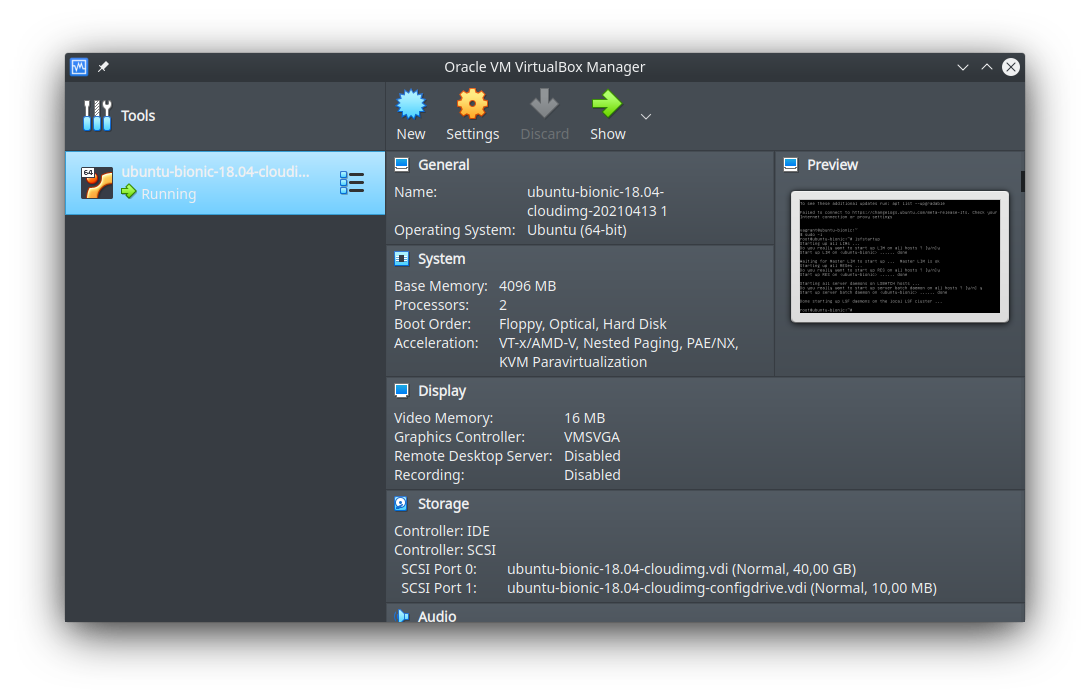
\includegraphics[width=\linewidth]{vbox.png}
    \caption{VirtualBox}
    % \label{fig:block-scheme}
\end{figure}

\begin{figure}[h]
    \centering
    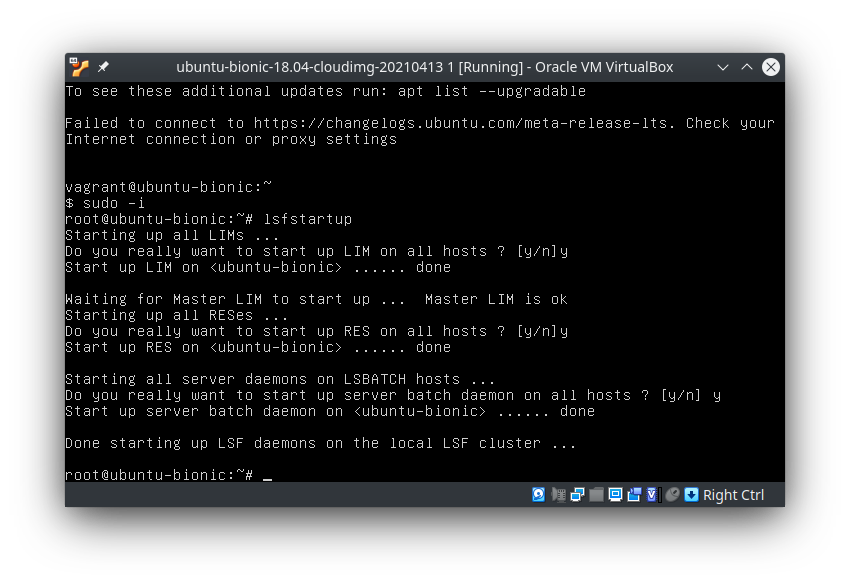
\includegraphics[width=\linewidth]{vm.png}
    \caption{Виртуальная машина. Изображен запуск LSF}
    % \label{fig:block-scheme}
\end{figure}

\begin{figure}[h]
    \centering
    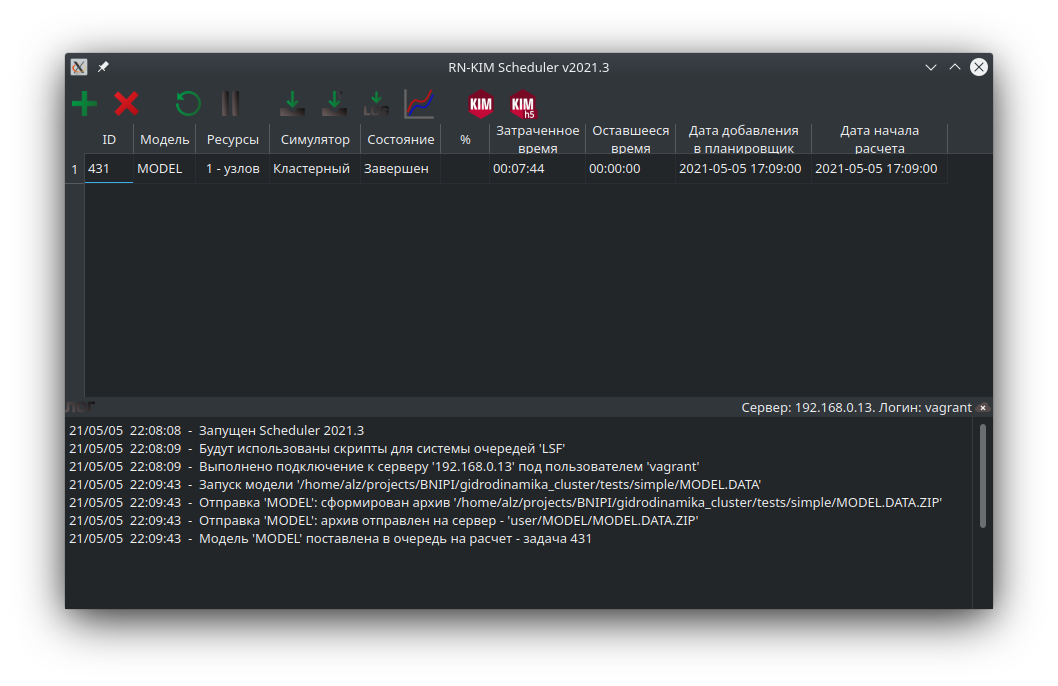
\includegraphics[width=\linewidth]{type_cluster.png}
    \caption{Скриншот Scheduler. Тип расчета модели: кластерный}
    % \label{fig:block-scheme}
\end{figure}

\begin{figure}[h]
    \centering
    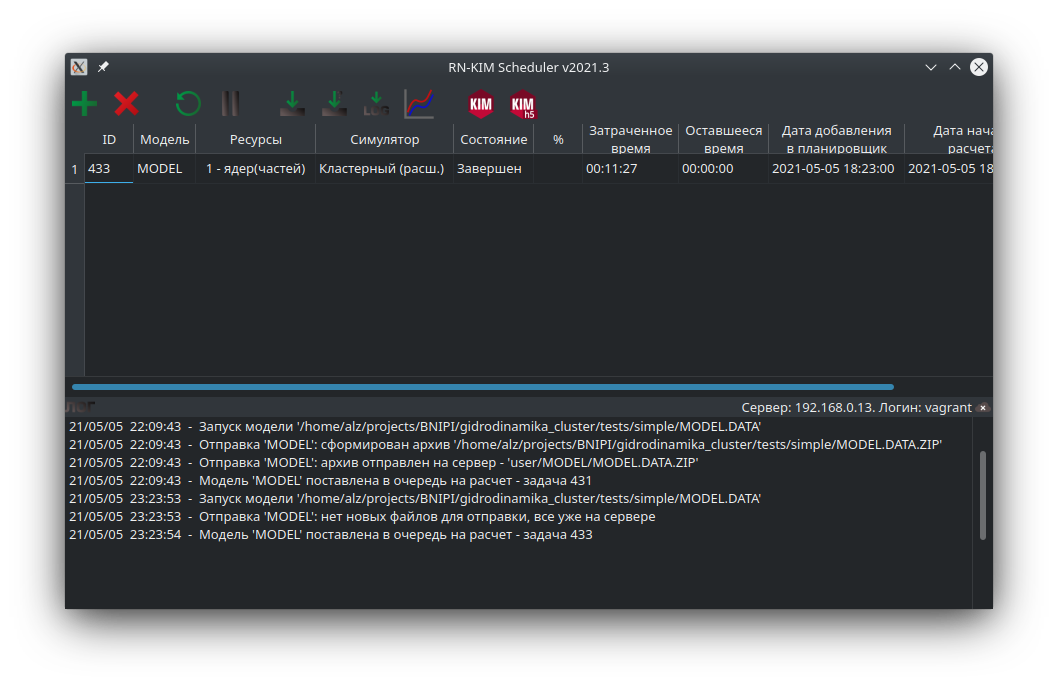
\includegraphics[width=\linewidth]{type_cluster_expanded.png}
    \caption{Скриншот Scheduler. Тип расчета модели: кластерный (расш.)}
    % \label{fig:block-scheme}
\end{figure}

\begin{figure}[h]
    \centering
    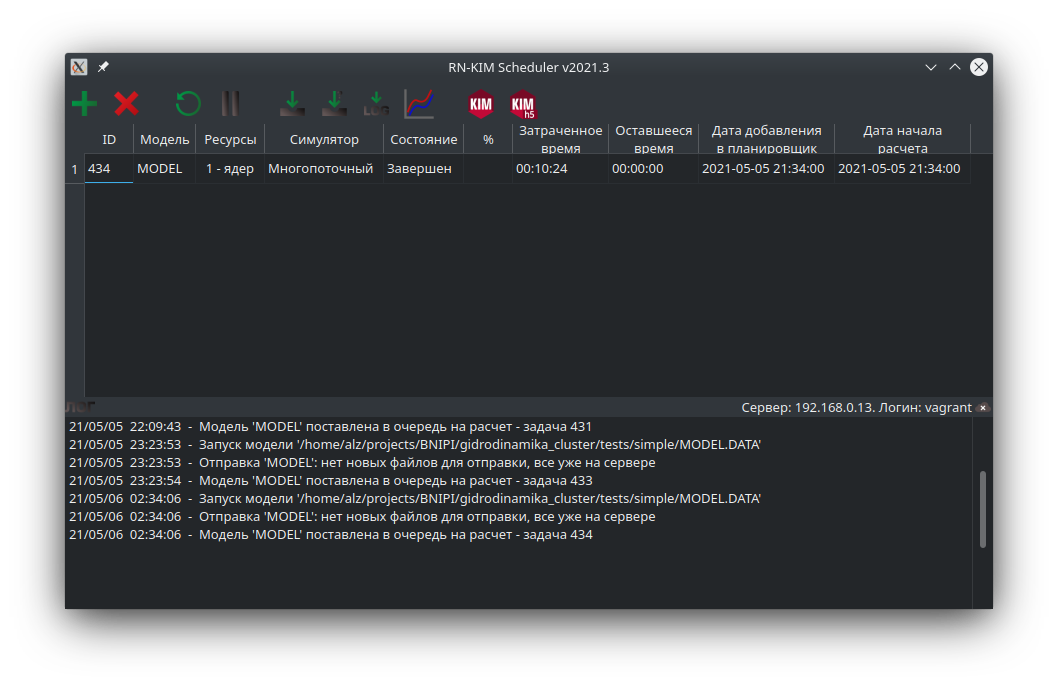
\includegraphics[width=\linewidth]{type_multithread.png}
    \caption{Скриншот Scheduler. Тип расчета модели: многопоточный}
    % \label{fig:block-scheme}
\end{figure}

\begin{figure}[h]
    \centering
    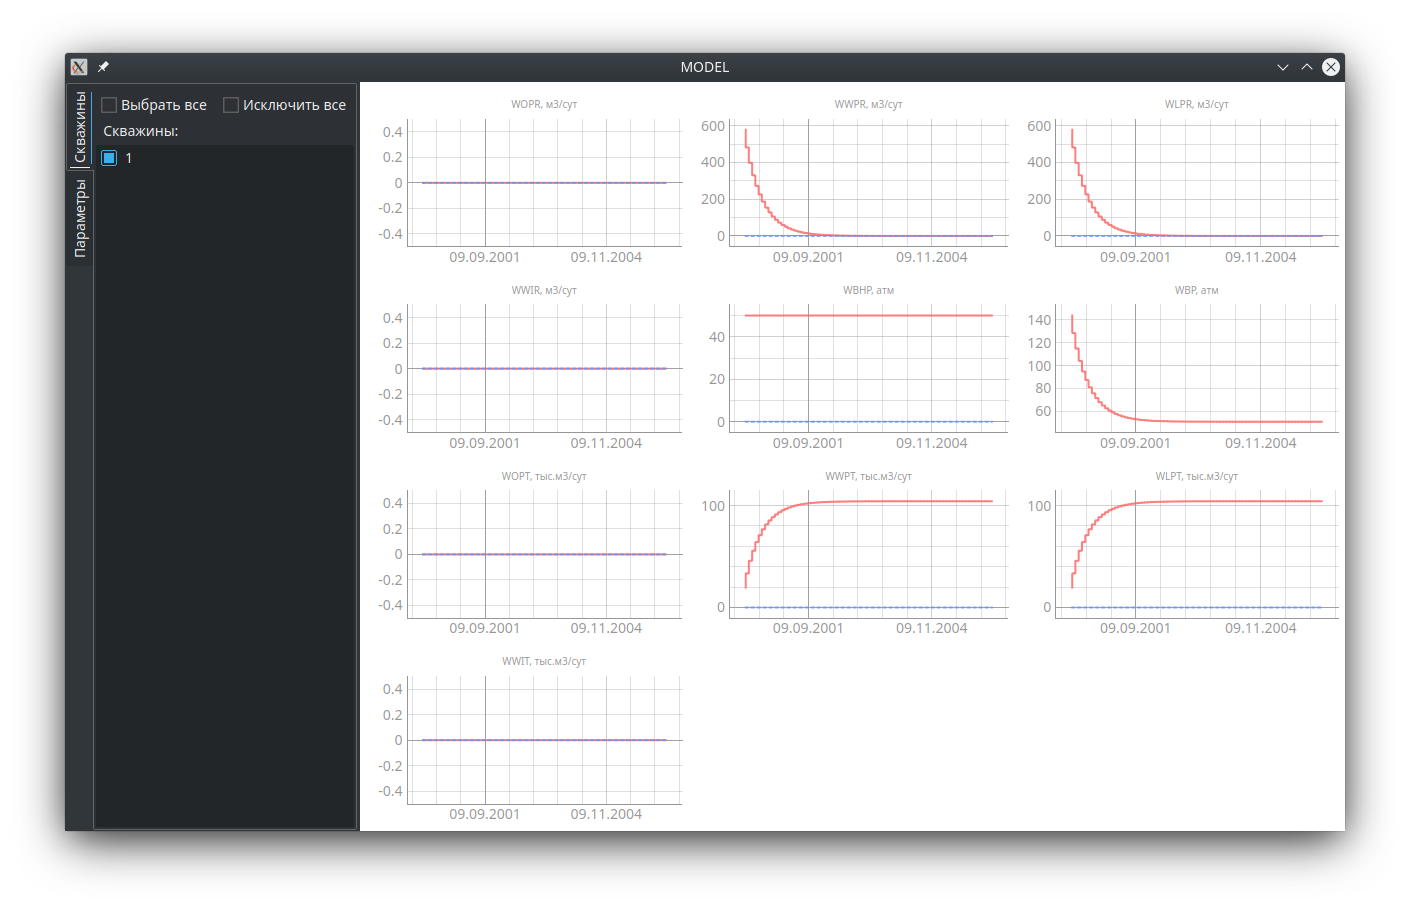
\includegraphics[width=\linewidth]{curves.png}
    \caption{Скриншот Scheduler. Рассчитанные кривые модели}
    % \label{fig:block-scheme}
\end{figure}

\clearpage